% DO NOT COMPILE THIS FILE DIRECTLY!
% This is included by the other .tex files.

\begin{frame}
\titlepage
\end{frame}

\begin{frame}
  \frametitle{What changed since the last workshop?}
  \begin{itemize}
    \item ATT\&CK has been steadily on the rise
    \item We have observerd it becoming a {\bf baseline for contextualisation} in several communities
    \item Relatively {\bf simple} to understand
    \item Makes the {\bf ingestion} of data based on context much easier
    \item Its use boosts {\bf analytical use-cases} (risk assessment, threat intelligence)
    \item This made us think about how we could further capitalise on its success
  \end{itemize}
\end{frame}

\begin{frame}
  \frametitle{New ATT\&CK sighting reporting format}
  \begin{itemize}
    \item Result of discussions with MITRE
    \item MISP server hosts can now decide to export an {\bf enumeration of the patterns} used based on the data-set
    \item Subject to all regular {\bf restSearch filtering methods} (time, organisation, context, etc)
    \item Export returns the data-set in MITRE's owns {\bf ATT\&CK sighting format}
  \end{itemize}
\end{frame}

\begin{frame}
  \frametitle{Searching our data-set for ATT\&CK-like matrix heatmaps}
  \begin{itemize}
    \item new standard {\bf restSearch return format}
    \item Returns {\bf HTML navigator-like heatmap}
    \item Easy integration into existing web applications
    \item Make use of all the MISP API filtering options
    \item Interested in how the rest of your {\bf sector} shapes up?
    \item Or perhaps different {\bf time} frames?
    \item Why not both and {\bf compare} them?
  \end{itemize}
\end{frame}

\begin{frame}
  \frametitle{Searching our data-set for ATT\&CK-like matrix heatmaps}
  \begin{itemize}
    \item The full dataset for a given time in an instance
  \end{itemize}
  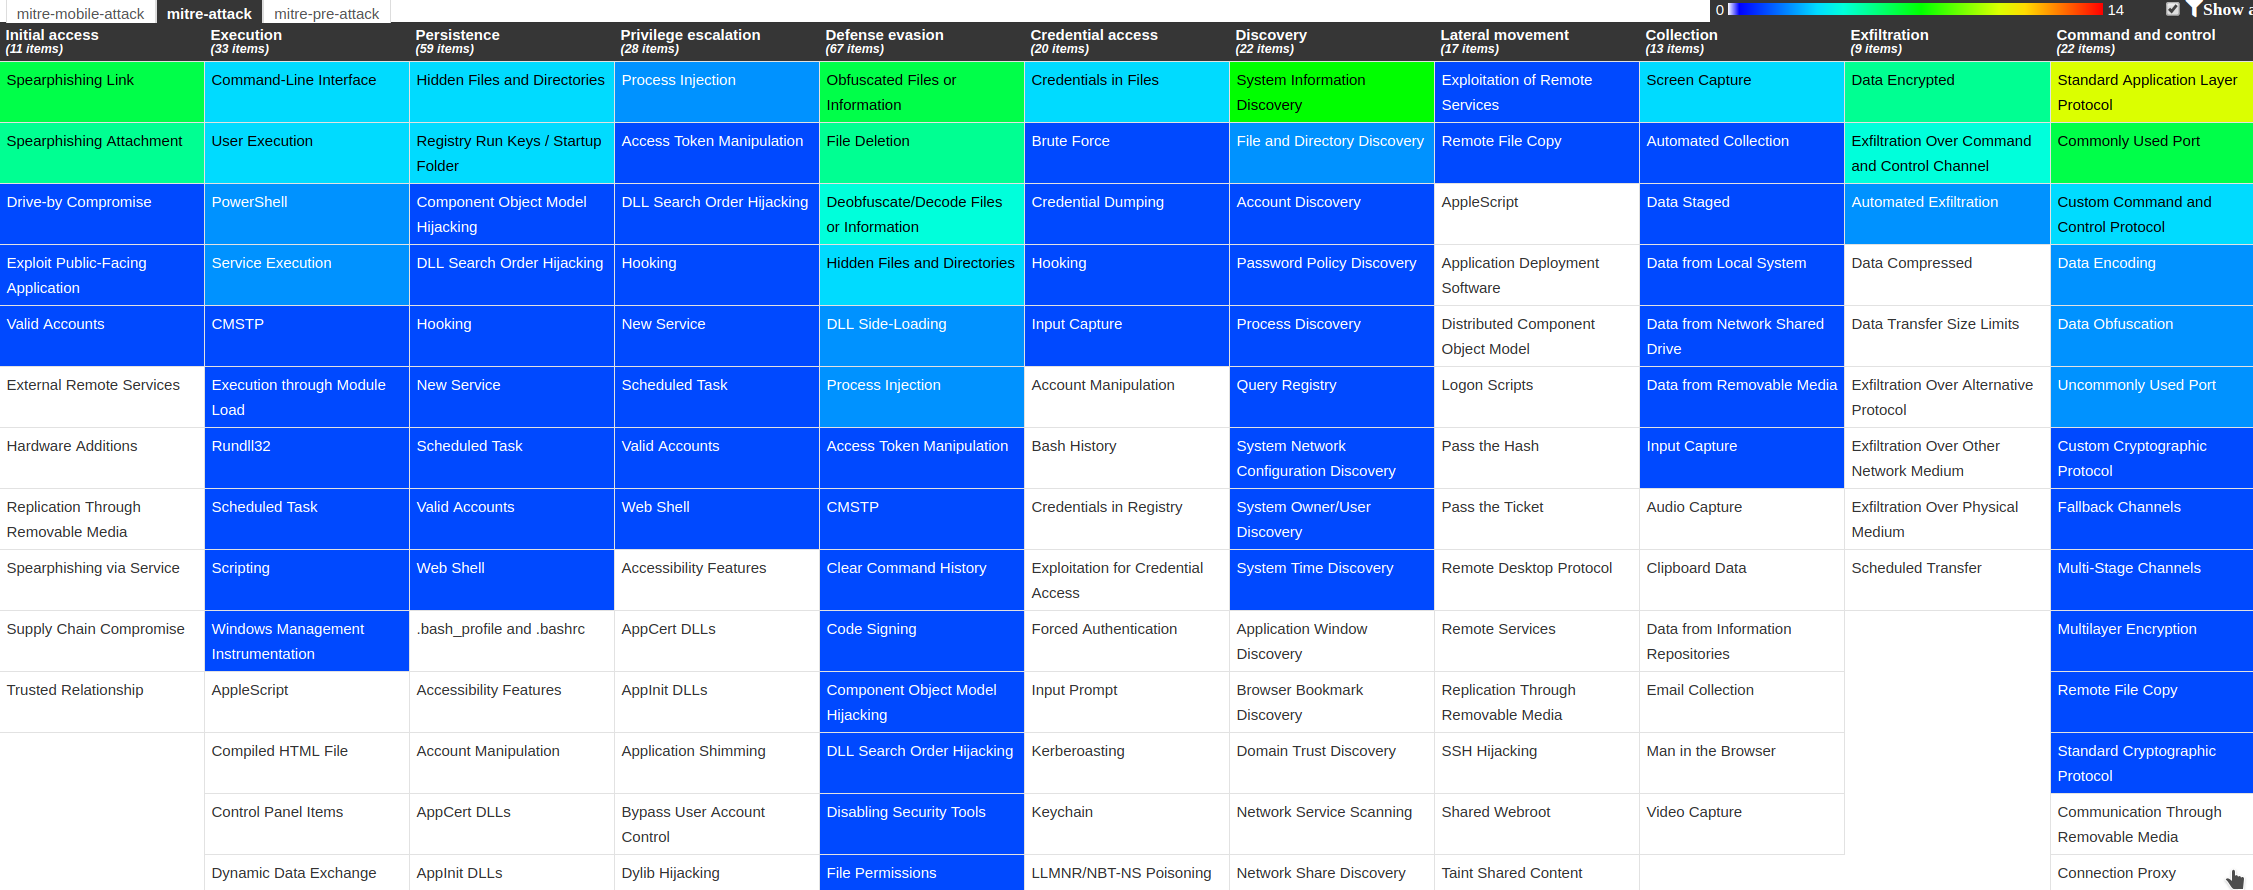
\includegraphics[scale=0.18]{matrix.png}
\end{frame}

\begin{frame}
  \frametitle{Searching our data-set for ATT\&CK-like matrix heatmaps}
  \begin{itemize}
    \item The full dataset for a given time in an instance
  \end{itemize}
  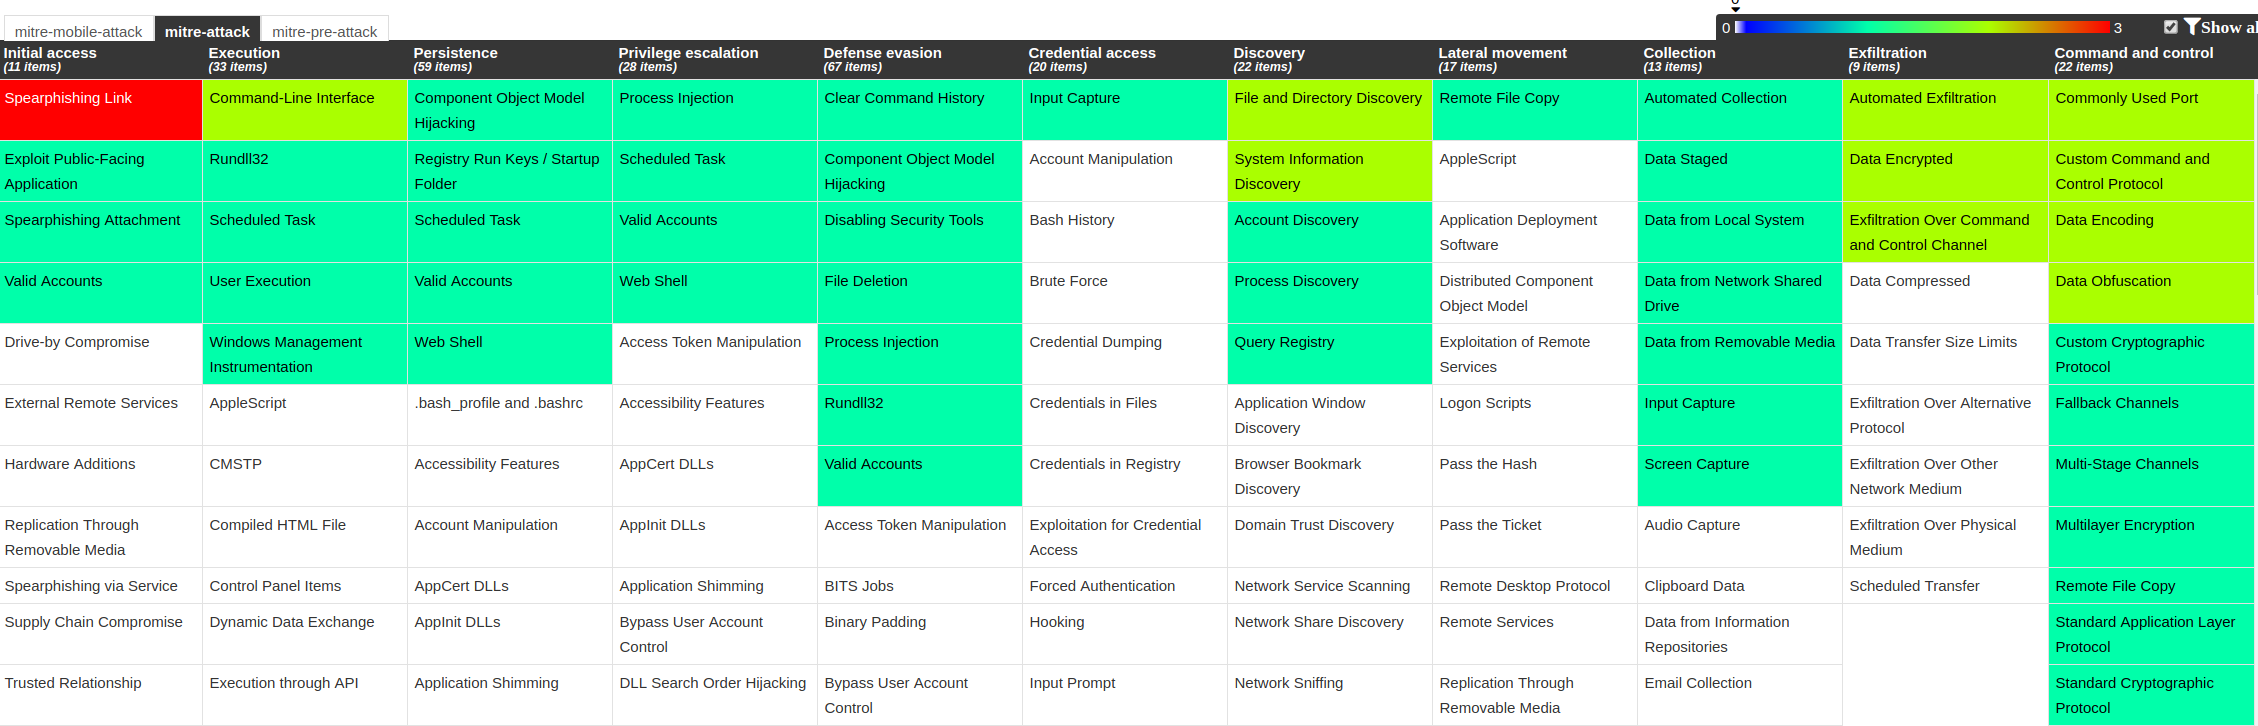
\includegraphics[scale=0.18]{matrix2.png}
\end{frame}

\begin{frame}
  \frametitle{ATT\&CK matrices as a standardised methodology}
  \begin{itemize}
    \item The advent of ATT\&CK had a secondary effect that was somewhat anticipated
    \item {\bf Francesco Bigarella} from ING showcased {\bf attack4fraud}
    \begin{itemize}
      \item {\bf ATT\&CK like matrix}
      \item Makes use of kill-chain phases
      \item Enables all of the advantages provided by the framework (such as technique frequency analysis)
    \end{itemize}
    \item This inspired us to allow for other matrix-like galaxies to be added
  \end{itemize}
        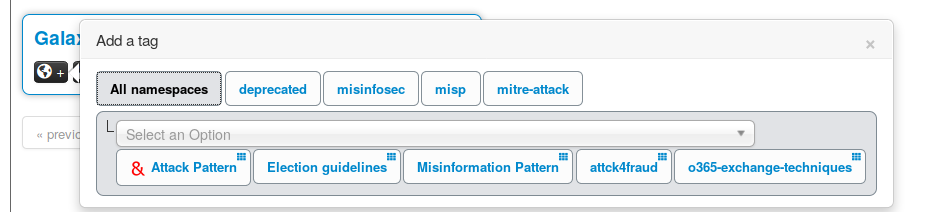
\includegraphics[scale=0.3]{matrix-like.png}
\end{frame}


\begin{frame}
  \frametitle{ATT\&CK matrices as a standardised methodology outcomes}
  \begin{itemize}
    \item Several ATT\&CK like matrices added since in MISP galaxy
    \begin{itemize}
      \item {\bf attck4fraud}
      \item {\bf Election guidelines}
      \item {\bf Office365 exchange techniques}
      \item {\bf AM!TT Tactic}\footnote{\url{https://github.com/misinfosecproject/amitt_framework}} (Adversarial Misinformation and Influence Tactics and Techniques) framework for describing disinformation incidents
    \end{itemize}
  \end{itemize}
\end{frame}

\begin{frame}
  \frametitle{Election guidelines}
  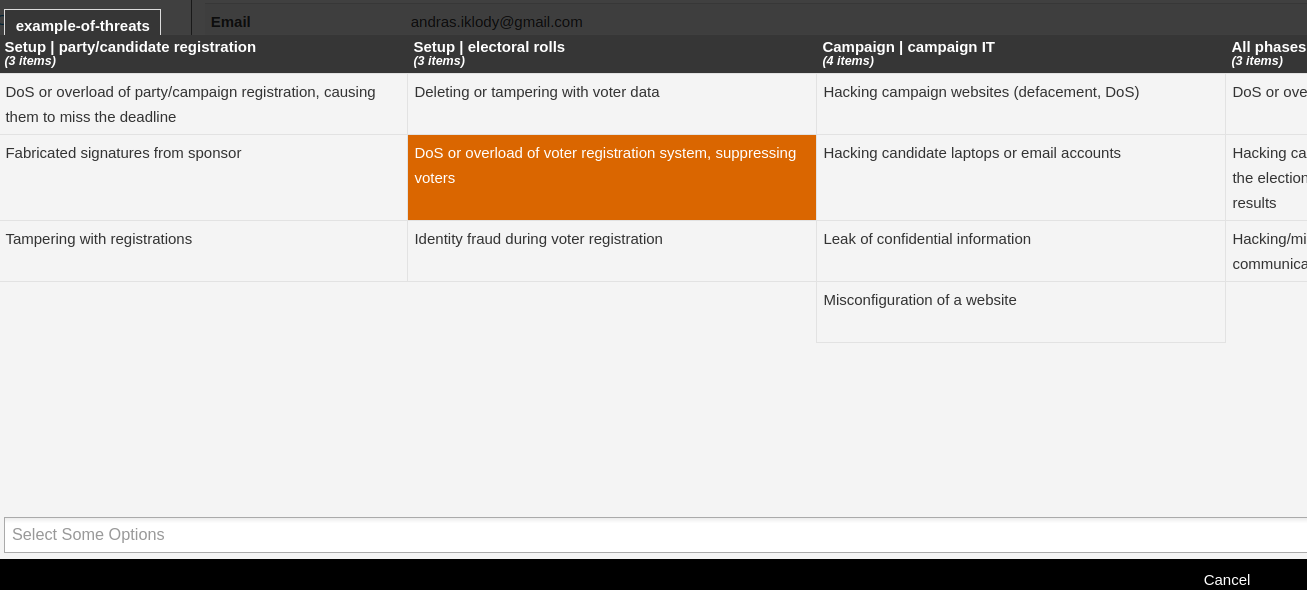
\includegraphics[scale=0.3]{election.png}
\end{frame}

\begin{frame}
  \frametitle{Office 365 techniques}
  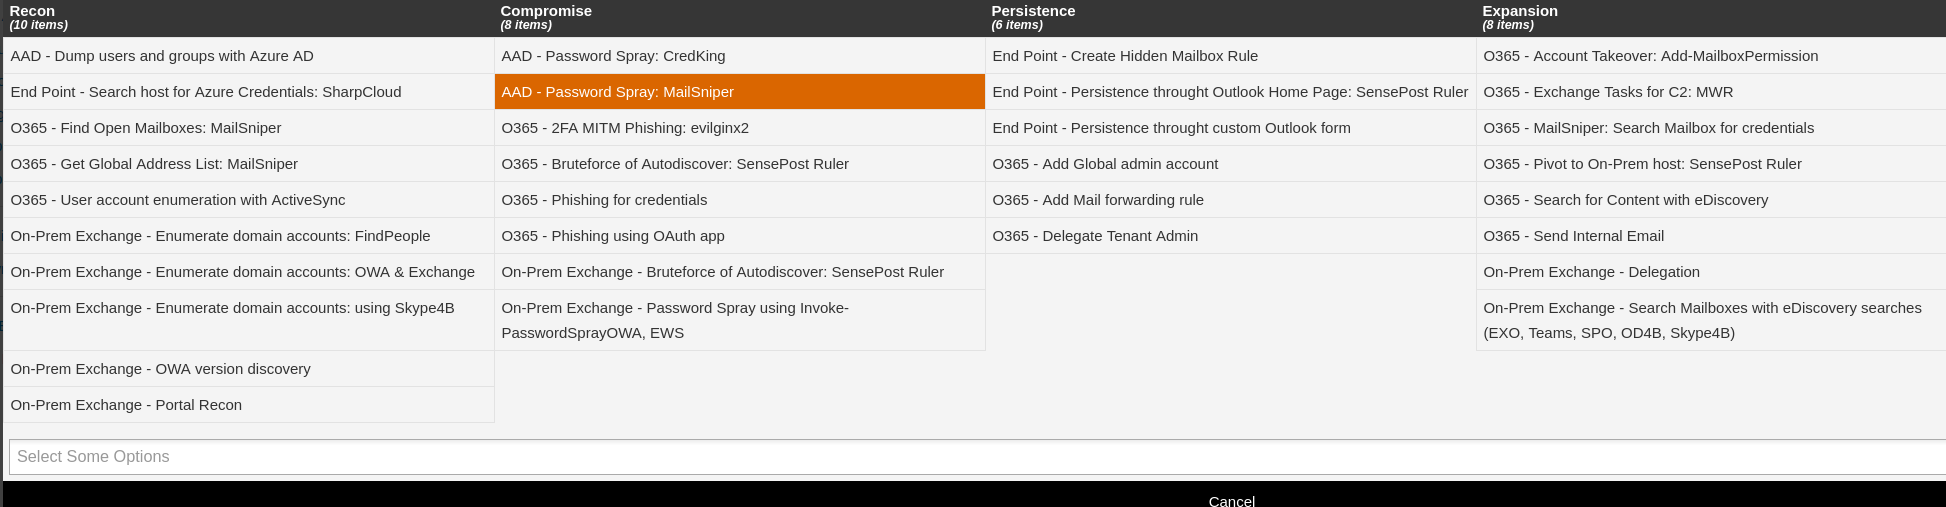
\includegraphics[scale=0.3]{office.png}
\end{frame}

\begin{frame}
  \frametitle{AM!TT Tactic (Adversarial Misinformation and Influence Tactics and Techniques)}
  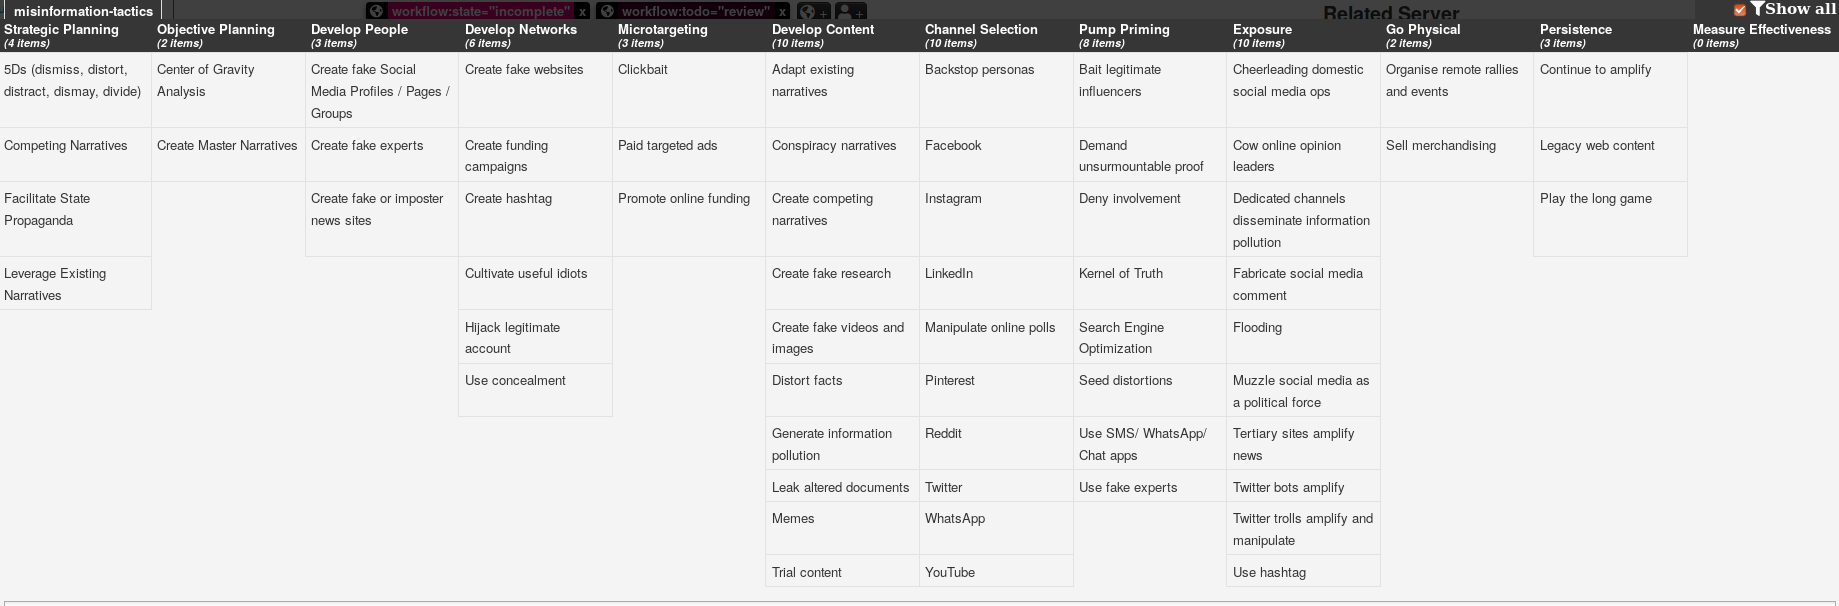
\includegraphics[scale=0.3]{amitt.png}
\end{frame}

\begin{frame}
        \frametitle{Conclusion}
        \begin{itemize}
                \item The matrix-like enhancement from the MISP galaxy format will be added in the default MISP galaxy standard format\footnote{\url{https://www.misp-standard.org/}}
                \item MITRE ATT\&CK sighting export in MISP was a first step to automate sharing of sightings ($\rightarrow$ public/private repository of sightings)
                \item ATT\&CK like matrices become more and more common, thanks the {\bf continuous work of the community}
        \end{itemize}
\end{frame}

